\documentclass[aspectratio=169]{beamer}

\usepackage[utf8]{inputenc}
\usepackage{soul}
%\usepackage{pdfpcnotes}
\usepackage{listings}

\usetheme{Hannover}
\usecolortheme{dove}

\AtBeginSection[]{
  \begin{frame}
  \vfill
  \centering
  \begin{beamercolorbox}[sep=8pt,center,shadow=true,rounded=true]{title}
    \usebeamerfont{title}\insertsectionhead\par%
  \end{beamercolorbox}
  \vfill
  \end{frame}
}

\lstset{language=C++,
                basicstyle=\ttfamily,
                keywordstyle=\color{blue}\ttfamily,
                stringstyle=\color{red}\ttfamily,
                commentstyle=\color{purple}\ttfamily,
                morecomment=[l][\color{magenta}]{\#}
}


\title{SoPra-Team-10}
\author{Server}
\date{\today}

\begin{document}
\maketitle

\begin{frame}
    \frametitle{Überblick}
    \begin{columns}
        \begin{column}{0.3\textwidth}
            \begin{center}
                \begin{figure}[H]
                    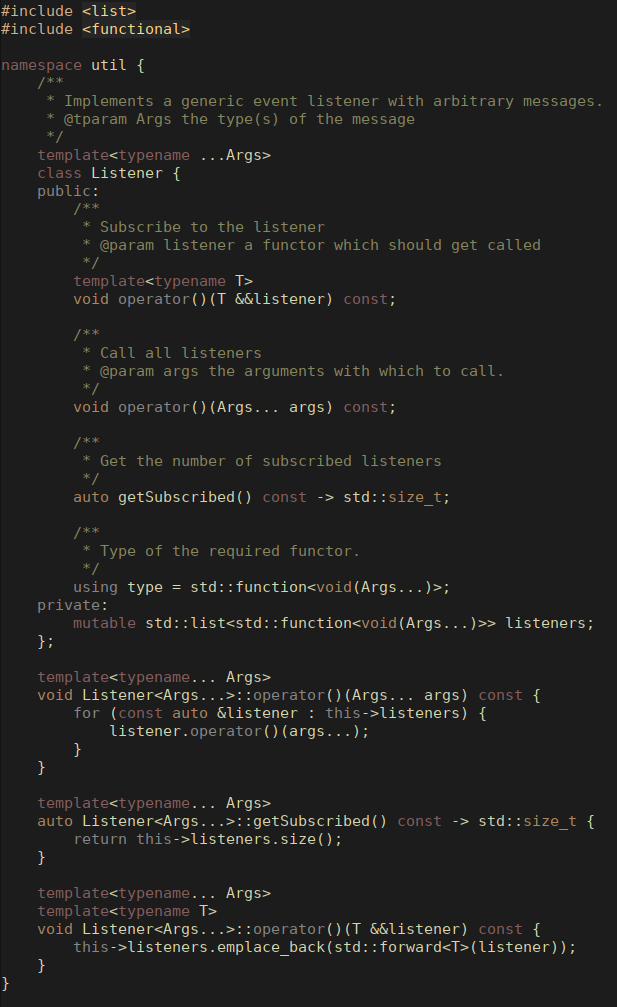
\includegraphics[height=6cm]{screenshot.png}
                \end{figure}
            \end{center}
        \end{column}
        \begin{column}{0.7\textwidth}
            \begin{itemize}
                \item Vollständig in C++17 geschrieben
                    \pause
                \item Modularer Aufbau (Trennung in Network-, Messages-, GameLogic- und Serverkomponente)
                    \pause
                \item MVC
                    \pause
                \item Replay implementiert
                    \pause
                \item Alle Mods implementiert
                    \pause
                \item Mehrere zeitgleiche Spiele
            \end{itemize}
        \end{column}
    \end{columns}
\end{frame}

\begin{frame}
    \frametitle{Krasse Features}
    \begin{itemize}
        \item 167 Unit Tests %TODO update me
            \pause
        \item Mit Doxygen dokumentiert
            \pause
        \item Statische und Dynamische Analyse (Clang-Tidy und Address-Sanitizer)
            \pause
        \item Fertiges Docker-Image
            \pause
        \item CI (Testen des Docker-Images, Unittests (mehrfache Wiederholung in unterschiedlicher Reihenfolge))
            \pause
        \item Ausführliches README mit Anleitung zum Installieren und Nutzen
    \end{itemize}
\end{frame}

\end{document}
